\documentclass[12pt,a4paper]{article}
\usepackage[utf8]{inputenc}
\usepackage{a4wide}
\usepackage[spanish,es-tabla]{babel}
\usepackage[spanish]{babel}
\usepackage{amsmath}
\usepackage{amsthm}
\usepackage{booktabs}
\usepackage{multirow} 
\usepackage{placeins}
\usepackage{hyperref}
\usepackage{fancyhdr}
\usepackage{titling}
\usepackage[T1]{fontenc}
\usepackage{graphicx}
\usepackage{floatrow}
\usepackage{siunitx}
\usepackage{listings}
\usepackage{minted}
\usepackage[table,xcdraw]{xcolor}
\usepackage{subcaption}
\usepackage{ragged2e}
\setminted[C]{fontsize=\footnotesize, tabsize=4}
\setminted[make]{fontsize=\footnotesize, tabsize=4}
\setminted[gas]{fontsize=\footnotesize, tabsize=2}
\setminted[bash]{fontsize=\footnotesize, tabsize=4}


\graphicspath{{images/}}

\newfloatcommand{capbtabbox}{table}[][\FBwidth]
\newcommand{\rulesep}{\unskip\ \vrule\ }

\sisetup{
locale=DE,
per-mode=fraction,
separate-uncertainty,
% exponent-to-prefix,
% prefixes-as-symbols=false,
list-units=brackets,
range-units=brackets,
multi-part-units=brackets,
table-unit-alignment=left,
% load=prefixed,
load-configurations=abbreviations,
}

\newcommand{\thetitle}{Trabajo Práctico 2: Machine Learning}
\newcommand{\theauthor}{Pérez Andrade Violeta\\Sinisi Fernando}
\newcommand{\thedate}{Segundo Cuatrimestre de 2020}

\hypersetup{
    unicode=false,
    pdftoolbar=true,
    pdfmenubar=true,
    pdffitwindow=false,
    pdftitle={\thetitle},
    pdfsubject={},
    pdfkeywords={6620-Organización de Datos},
    colorlinks=true,
    linkcolor=black,
    citecolor=black,
    filecolor=magenta,
    urlcolor=cyan
}

%%%%%%%%%%%%%%%%%%%%%%%%%%%%%%%%%%%%%%%%%%%%%%%%%%%%%%%%%%


\pagestyle{fancy}
\fancyhf{}
\lhead{Trabajo Práctico 2}
\rhead{Organización de Datos}
\cfoot{\thepage}

\setlength{\headheight}{14.5pt}


\begin{document}


\begin{titlepage}
	\centering
    \vspace*{2.5cm}

    
\includegraphics[scale = 0.7]{imgs/logofiuba.jpg}\\[2.0 cm]

	\textsc{\Large 75.06 Organización de Datos}\\[0.7 cm]
	\textsc{Facultad de Ingeniería, Universidad de Buenos Aires}\\[0.5 cm]

	\rule{0.94\linewidth}{0.2 mm} \\[0.4 cm]
	{\huge \bfseries \thetitle}\\
	\rule{0.94\linewidth}{0.2 mm} \\[1.2 cm]

    \begin{tabular}{lll} % Datos del alumno
        \toprule
        Padrón & Alumno & Dirección de correo \\
        \midrule
        101456 & Pérez Andrade, Violeta  & viperez@fi.uba.ar \\
        99139 & Sinisi, Fernando & fsinisi@fi.uba.ar \\
        \bottomrule
    \end{tabular}\\


    \vspace*{1cm}

\end{titlepage}

\tableofcontents
\newpage

\section{Introducción}

El objetivo principal del trabajo práctico es construir un modelo capaz de estimar la probabilidad de éxito para cada oportunidad de negocio de la empresa frío-frío, con el menor error posible. El error de la solución (inversamente: su calidad) es calculado con la ecuación de log-likelihood:
\begin{equation}
\operatorname{loss}(\mathbf{y}, \hat{\mathbf{y}})=-\frac{1}{N} \sum_{i=1}^{N} y_{i} \log \left(\hat{y}_{i}\right)+\left(1-y_{i}\right) \log \left(1-\hat{y}_{i}\right)
\end{equation}
siendo \textit{y} un vector binario con el éxito real de cada oportunidad y \textit{ŷ} un vector con las probabilidades continuas. \\
Este modelo, se realizo con algoritmos de Machine Learning, lo cual busca poder generar clasificaciones en base a un entrenamiento sobre información pasada, las cuales luego son validadas. En el presente trabajo se probaron distintos algoritmos, los cuales hacen uso de los datos en distinta manera. Por esto ultimo es muy importante saber cuales datos usar y como codificarlos. \\
De esta forma, fueron brindados dos sets de datos: 
\textit{Train\_TP2\_Datos\_2020-2C.csv} y \textit{Test\_TP2\_Datos\_2020-2C.csv} los cuales fueron utilizados, respectivamente, para entrenar los modelos, y luego realizar las predicciones. \\
En ambos sets de datos, cada fila representa un ítem
vendido para una ’oportunidad’ la cual consiste en un proyecto de venta o instalación de equipos para un cliente. La venta se estructura alrededor de TRF (Toneladas de refrigeración) y puede ser una oportunidad que resultó exitosa o no. \\
El código correspondiente se puede hallar en el siguiente repositorio: \url{https://github.com/FernandoSinisi/Orga-Datos-2C-2020}
\newpage
  

\section{Limpieza de datos}
La limpieza de los datos es un proceso fundamental para identificar datos aberrantes, faltantes o atípicos. Para el caso del set de datos utilizado en este trabajo, en el primer trabajo practico notamos que había ciertas columnas cuyo contenido era nulo en mas del 60\% de su totalidad. Las mismas son:
\begin{itemize}
    \item Last\_Activity
    \item Actual\_Delivery\_Date
    \item Price
    \item Size
    \item Product\_Type
    \item Brand
    \item Product\_Category\_B
    \item Source 
\end{itemize}
Por otra parte, la columna Sales\_Contract\_No no se utilizo dado que se advirtió que la misma contenía un leak del target. \\
Una vez eliminadas estas columnas, quedaron algunos datos vacíos pero no en gran cantidad, por lo que, para ciertos algoritmos que no podían entrenar/predecir con datos faltantes, se opto por reemplazar los mismos con 0.

\section{Feature Engineering}
Se buscaron todos los atributos o relaciones posibles de las variables contenidas en el set de
datos proporcionado para el trabajo para luego realizar una selección de features y poder utilizar los mas relevantes para los algoritmos a aplicar.\\
De esta forma, a partir de los features ya existentes se agregaron lo siguientes:
\begin{itemize}
    \item Diferencia en días: Indica la diferencia, en días, entre la fecha de creación de la oportunidad y la ultima modificación de la misma.
    \item A partir de los features de tipo fecha:
    \begin{itemize}
        \item Planned\_Delivery\_End\_Date
        \item Planned\_Delivery\_Start\_Date
        \item Quote\_Expiry\_Date
        \item Opportunity\_Created\_Date
        \item Last\_Modified\_Date
    \end{itemize}
    para cada uno, se crearon dos columnas: DOY y Year las cuales representan, respectivamente, el día de año y el año de la fecha.
\end{itemize}
\subsection{Feature Selection}
\section{Feature Encoding}
Después del analisis del primer trabajo practico, se evidencio que el set de datos consiste de variables de tipo numéricas, las cuales no necesitan ningún tipo de codificación, y por otra parte variable categórica. Como no hay ninguna variable de tipo \textbf{string}, se investigo cual era la mejor forma de tratar este tipo de variables(categóricas), y para ello, se utilizaron los encodings que se detallan a continuación:

\subsection{Mean encoding}
\subsection{Binary Encoding}
\subsection{Count Encoder}
\subsection{GLMM Encoder}
\subsection{Hashing Encoder}
\subsection{Helmert Encoder}
\subsection{JamesStein Encoder}
\subsection{LeaveOneOut Encoder}
\subsection{MEstimate Encoder}
\subsection{Ordinal Encode}
\subsection{Sum Encoder}
\subsection{Polynomial Encoder}
\subsection{OE Encoder}
\subsection{OneHot Encoder}
\subsection{Catboost Encoder}
\subsection{Base N Encoder}
\section{Modelos}
\subsubsection{KNN}
Este algoritmo consiste en encontrar los vecinos más cercanos al punto que se busca clasificar, para luego predecir la clase del punto en cuestión que se obtendrá a partir de la clase mayoritaria presente en sus vecinos.
Los hiperparámetros comunes en KNN son:
\begin{itemize}
    \item n-neighbors: Radio del círculo para la clasificación de los puntos.
    
    \item weights: Puede seleccionarse entre \textit{uniform}, donde cada vecino dentro del perímetro tiene el mismo peso o "distancia", donde los puntos mas cercanos tendrán un mayor peso.
    
    \item metric: Define la metrica para calcular las distancias entre los puntos.
    
\end{itemize}
KNN es uno de los algoritmos mas sencillos de Machine Learning pero definiendo correctamente sus hiperparámetros puede ser muy eficiente. Una desventaja es que se trata de un algoritmo de orden cuadrático por lo que puede tener un gran impacto a la hora de la ejecución.

\subsection{Algoritmos de clasificacion}

\subsubsection{Random Forest}
Este es uno de los algoritmos mas populares para clasificación, el cual crea un conjunto de árboles de decisión a partir de un subconjunto del set de datos de entrenamiento seleccionado al azar. 
Luego, para decidir la clase final del objeto puede utilizar dos formas de decisión, por mayoría de votos o por peso (donde los árboles con alta tasa de error reciben un valor de bajo peso y viceversa, permitiendo que los árboles con baja tasa de error tengan mayor impacto).
Los hiperparámetros comunes en RandomForest son:

\begin{itemize}
    \item n-estimators: Número de árboles.
    
    \item max-features: Cantidad de features a considerar en cada partición del árbol.
    
    \item max-depth: Profundidad de cada árbol.
    
    \item min-samples-split: Cantidad mínima de muestras requeridas para realizar una partición del árbol.
    
    \item min-samples-leaf: Cantidad minima de muestras por cada hoja del arbol
    
    \item bootstrap: Método de selección de muestras para el entrenamiento de cada árbol.
    
\end{itemize}

\subsubsection{SVC}
El objetivo de SVC, es entrenar el set de datos encontrando el mejor hiper-plano que divide a los mismos en categorías.

\subsubsection{NuSVC}
Este algoritmo es similar a SVC (Support Vector Classifier), con la diferencia de que usa como parámetro "nu" el cual controla el número de vectores soportados.

\subsubsection{Naive Bayes Classifier}
Este algoritmo considera cada feature de forma independiente, calculando la probabilidad de que el feature pertenezca a cada una de las categorías, dando como resultado la que contenga el mayor valor de probabilidad. El modelo utilizado para calcular dicha probabilidad esta basado en el teorema de Bayes. Se parte de la suposición de que todos los predictores tienen el mismo efecto en el resultado. Existen diferentes tipos de clasificadores que siguen este modelo.

Los hiperparámetros comunes en Naive Bayes son:
\begin{itemize}
    \item alfa: Parámetro utilizado para realizar el suavizado de Laplace, el cual permite no tener probabilidades nulas a la hora de calcular la probabilidad de que el vector de palabras para un documento se encuentre en alguna de las categorias. Permitiendo siempre generar alguna clasificación. 
\end{itemize}

\subsubsection{XGBoost}
Este algoritmo, es un boosting de arboles de decisión en el cual, cada árbol intenta corregir lo que el anterior no pudo predecir correctamente. A partir de la combinación de varios árboles de decisión, logra buenas predicciones. Boosting es una técnica que funciona según el principio de ensamble. Combina un set de modelos débiles y mejora la precisión de la predicción.\\
Tiene una función objetivo que depende de los parámetros que tiene que aprender. La parte de la predicción esta dada por la diferencia entre el valor de la predicción y el valor real. La predicción final de un boosting es la sumatoria de las predicciones de varios arboles. Una de las cosas que hace que este algoritmo sea tan rápido es que únicamente recibe valores numéricos.
 
Los hiperparametros mas importantes son:
 \begin{itemize}
    \item n-estimators: Número de árboles.
    
    \item learning\_rate: Parametro de contracción. Escala los pesos agregados por un factor n  después de cada paso del árbol, reduce la influencia de cada árbol individual y deja espacio para que los  árboles futuros mejoren el modelo. Tambien sirve para evitar el overfitting.
    
    \item max-depth: Profundidad de cada árbol.
    
    \item objective: La función objetivo, se puede usar alguna de las ya disponibles(como por ejemplo 'binary:logistic', 'reg:linear', 'multi:softprob') o se le puede pasar una función propia.
    
    \item booster: Para seleccionar que booster usar, puede ser: gbtree, gblinear o dart.
    
\end{itemize}

\subsubsection{Red Neuronal}
Este algoritmo no lineal genera las predicciones a partir de la definición de una función de activación. Usualmente las funciones de activación mas comunes suelen ser: \textit{sigmoid}, \textit{relu} o \textit{softmax}. La combinación de distintas funciones de activación es lo que genera la red, donde se cuenta con una capa visible en la cual se reciben los inputs y distintas capas ocultas donde se procesa la información para obtener el output.

\begin{center}
    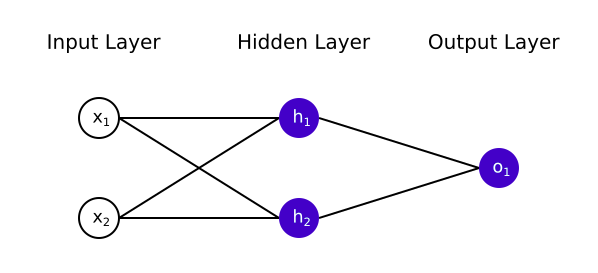
\includegraphics[scale=0.5]{imgs/red neuronal.png}
\end{center}

El objetivo de este algoritmo es el de disminuir el error cuadrático medio (\textit{loss}) para obtener mejores predicciones.
En particular, las redes utilizadas para el procesamiento de lenguaje natural son las Redes Neuronales Recurrentes las cuales, contienen loops en ellas para lograr la persistencia de la información. 

\begin{center}
    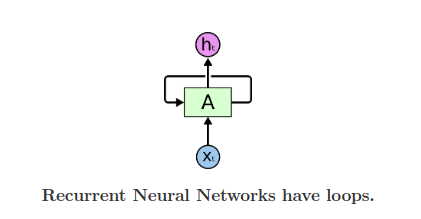
\includegraphics[scale=0.5]{imgs/red neuronal recurrente.png}
\end{center}

\subsubsection{LightGBM}
Este modelo es un algoritmo de \textit{gradient boosting} sobre arboles de decisión.
Produce el modelo predictivo a partir de un conjunto de modelos de predicción débiles. Construye el modelo de forma escalonada y lo generaliza disminuyendo la función de error creciendo verticalmente eligiendo la hoja con mayor "delta loss" para crecer. El crecimiento por hojas, en vez de por niveles, permite reducir aún más el \textit{loss}.

\begin{center}
    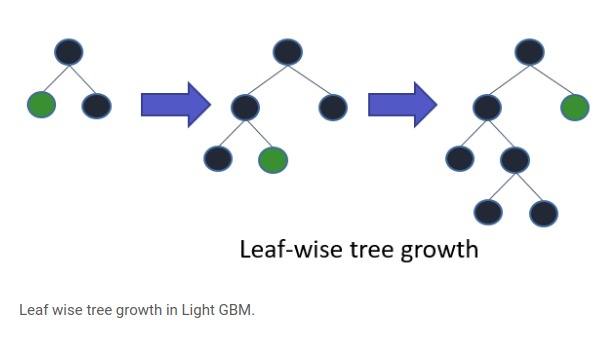
\includegraphics[scale=0.5]{imgs/lightgbm.jpeg}
\end{center}

\subsubsection{Logistic Regression}
Este modelo, es el método de referencia para problemas de clasificación binaria (aquellos donde solo existen dos valores de clase). El mismo, utiliza de base \textit{la función logística} o también llamada \textit{función sigmoidea}, la cual es representada como una curva en forma de S que puede tomar cualquier número real y asignarlo a un valor entre 0 y 1, pero nunca exactamente en esos límites. Logistic Regression predice la probabilidad de que un dato pertenezca a una clase (clase default) y luego esta predicción es transformada a un valor binario con la función logística. 
\section{Ensambles}
\section{Resultados Obtenidos}
\section{Conclusiones}
\end{document}
